\chapter{Results}
\label{chapter:results}

\section{Cache-oblivious B-tree}
We found the performance of cache-oblivious B-trees very competitive compared
to B-trees on both random uniform access patterns and modestly large working
sets. As seen on figure \ref{fig:cob-performance}, random \textsc{Find}s
were up to twice as fast in large cache-oblivious B-trees without ever being
significantly slower on small dictionaries.
The large density of the van Emde Boas tree is the likely reason for these
gains.
\textsc{FindNext} and \textsc{FindPrev} are also faster in cache-oblivious
B-trees.

\textsc{Insert} operations, however, are comparatively slow in
smaller cache-oblivious B-trees (e.g.\ $\leq$ 100~000 keys). We believe
this slowdown is probably due to the cost of rebuilds, which properly
amortizes away only on larger dictionaries. A smarter choice of tuning
constants (i.e.\ the minimum and maximum density and piece sizes) might
make updates of smaller dictionaries more efficient.

\begin{figure}
\centering
\begin{subfigure}[t]{0.45\textwidth}
	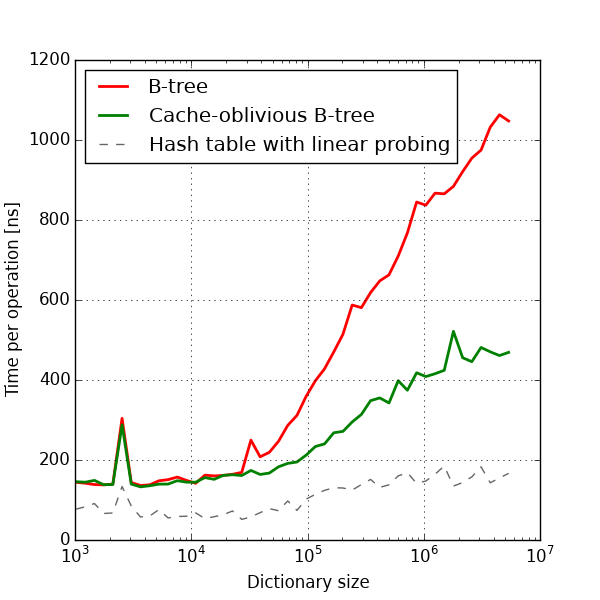
\includegraphics[width=\textwidth]{img/performance/cob-performance-1}
	\caption{Random \textsc{Find}s}
\end{subfigure}
~
\begin{subfigure}[t]{0.45\textwidth}
	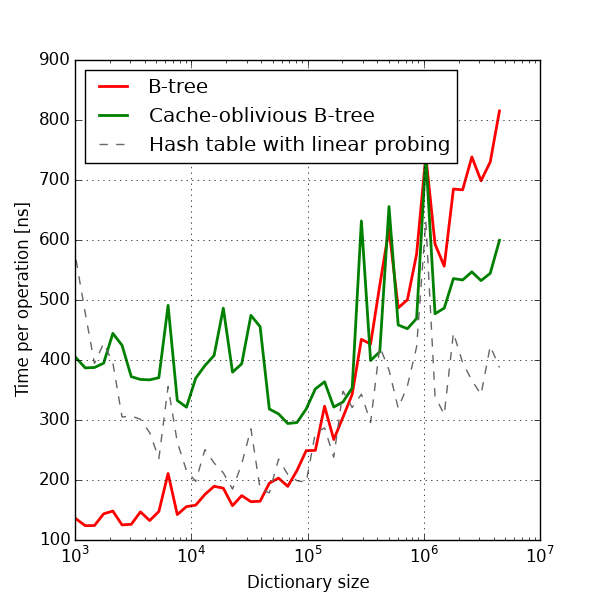
\includegraphics[width=\textwidth]{img/performance/cob-performance-2}
	\caption{Random \textsc{Insert}s}
\end{subfigure}
~
\begin{subfigure}[t]{0.45\textwidth}
	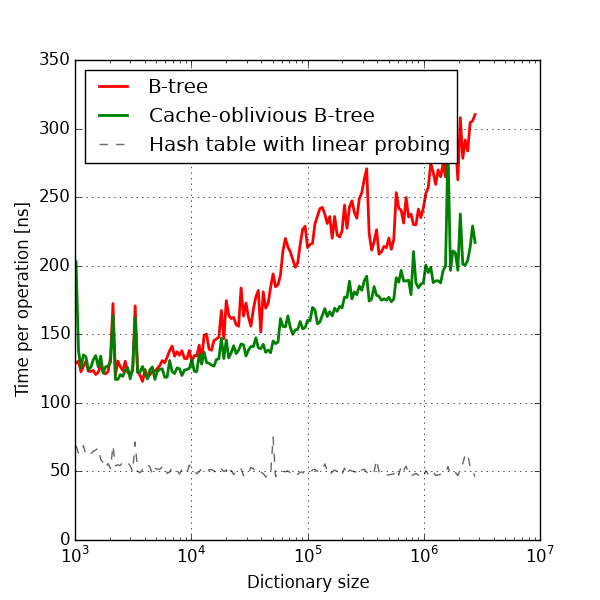
\includegraphics[width=\textwidth]{img/performance/cob-performance-3}
	\caption{\textsc{Find}s, working set of 1~000 keys}
\end{subfigure}
~
\begin{subfigure}[t]{0.45\textwidth}
	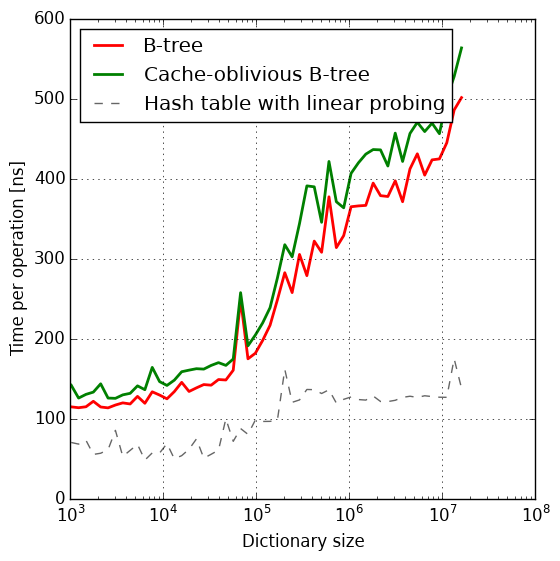
\includegraphics[width=\textwidth]{img/performance/cob-performance-4}
	\caption{\textsc{Find}s, working set of 100~000 keys}
\end{subfigure}
~
\begin{subfigure}[t]{0.45\textwidth}
	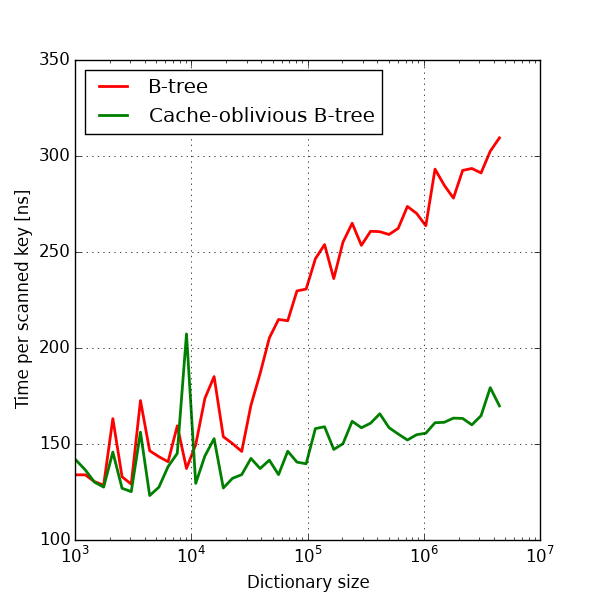
\includegraphics[width=\textwidth]{img/performance/cob-performance-5}
	\caption{Left-to-right scans over whole dictionary}
\end{subfigure}
~
\begin{subfigure}[t]{0.45\textwidth}
	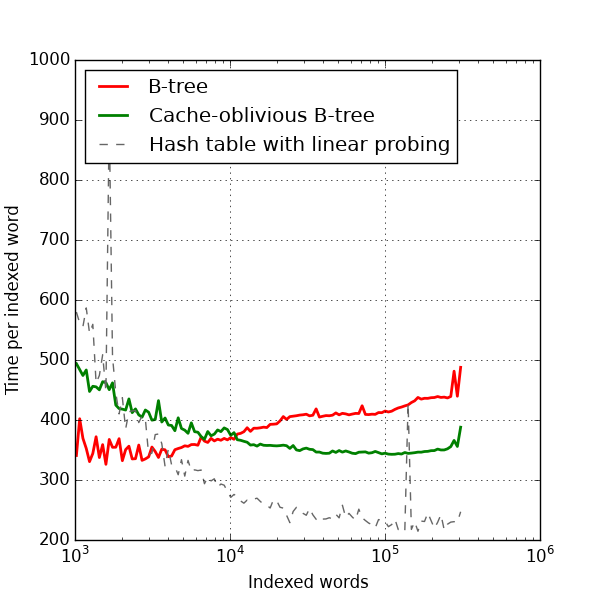
\includegraphics[width=\textwidth]{img/performance/cob-performance-6}
	\caption{Word occurrence counting}
\end{subfigure}
\caption{Benchmarks of cache-oblivious B-trees.
	Measurements of hash table with linear probing included for reference.}
\label{fig:cob-performance}
\end{figure}

\section{Self-adjusting structures}
Splay trees are the canonical self-adjusting structure we would like to
outperfrom. As expected, splay trees are somewhat slower than B-trees on
unpredictable operations (see Figure \ref{fig:self-adj-performance}).

\begin{figure}
\begin{subfigure}[b]{0.45\textwidth}
	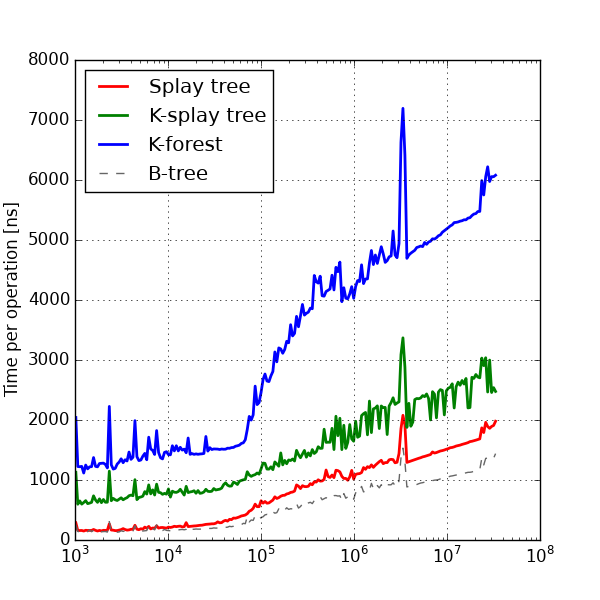
\includegraphics[width=\textwidth]{img/performance/self-adj-random-find}
	\caption{Random \textsc{Find}s}
\end{subfigure}
~
\begin{subfigure}[b]{0.45\textwidth}
	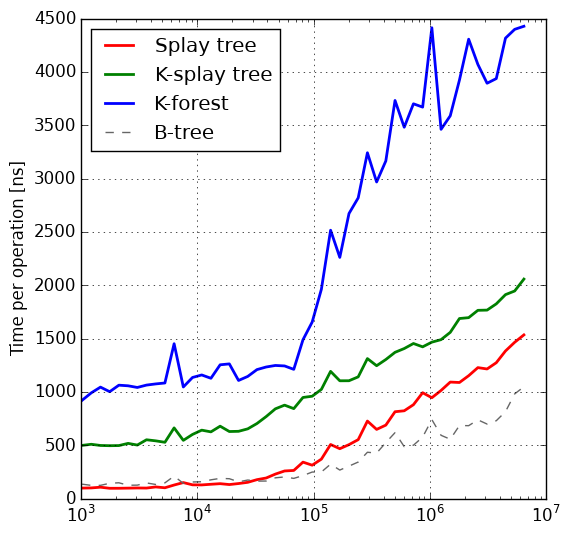
\includegraphics[width=\textwidth]{img/performance/self-adj-random-insert}
	\caption{Random \textsc{Insert}s}
\end{subfigure}
\\
\begin{subfigure}[b]{0.45\textwidth}
	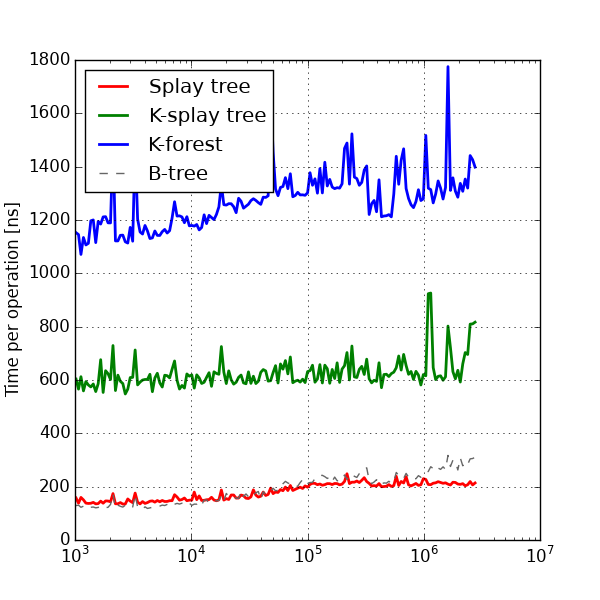
\includegraphics[width=\textwidth]{img/performance/self-adj-ws-1k}
	\caption{\textsc{Find}s, working set of 1~000 keys}
\end{subfigure}
~
\begin{subfigure}[b]{0.45\textwidth}
	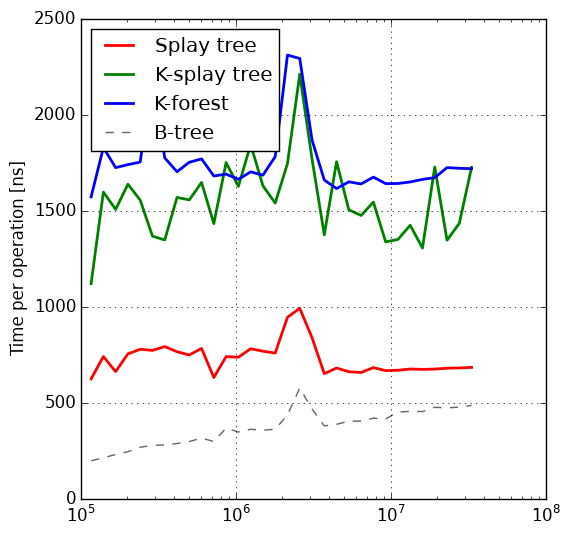
\includegraphics[width=\textwidth]{img/performance/self-adj-ws-100k}
	\caption{\textsc{Find}s, working set of 100~000 keys}
\end{subfigure}
% TODO: word occurrence counting
\caption{Benchmarks of self-adjusting structures.
	B-trees are included for reference.}
\label{fig:self-adj-performance}
\end{figure}

Unfortunately, we found both $k$-splay trees and $k$-forest lacking in
performance in every experiment.

Profiling $k$-splay trees showed that about 21\% of time is spent in
\texttt{ksplay\_walk\_to}, which finds the correct leaf for a key and puts the
path to the leaf into a buffer. About 37\% of the time is taken by
\texttt{ksplay\_step}, which performs a splaying step, along with helper
functions it calls (\texttt{flatten\_explore}, \texttt{compose\_twolevel}).

One suboptimal property of our implementation is that it dynamically
allocates the $k$-splayed path on every $k$-splay. Memory allocation alone
accounts for about 20\% of CPU time.
Keeping a global buffer for $k$-splayed paths could thus potentially bring
the performance of $k$-splay trees somewhat closer to splay trees.
As suggested in \cite{ksplay-sherk}, it should be possible to remove the
need to store the splayed path by top-down $k$-splaying.
Unfortunately, even with top-down $k$-splaying, every $k$-splay step needs
to touch $\Theta(k^2)$ keys and pointers, so we believe top-down $k$-splaying
would not significantly reduce the high cost of \texttt{ksplay\_step}.

Our measurements on small working sets confirm that splay trees, $k$-forests
and $k$-splay trees all have the working set property.

$k$-forests were slow both backed by B-trees and by cache-oblivious B-trees.
Choosing a larger $k$ slightly helped, but larger values of $k$ also degenerate
$k$-forests into their backing structure.

\section{Hashing}
\label{sec:hashing-results}
We compared a hash table with linear probing to a cuckoo hash table.
Both hash tables used a bytewise simple tabulation hash function.
The cuckoo hash table maintained a load factor between $\frac{1}{4}$ and
$\frac{1}{2}$ and the hash table with linear probing had a load factor
between $\frac{1}{4}$ and $\frac{3}{4}$.

Since cuckoo hash tables guarantee worst-case $\O(1)$ time for lookups,
we expected random \textsc{Find}s to be measurably slower with linear probing.
Linear probing lookups, however, performed almost exactly the same as
with cuckoo hashing, even with a higher load factor (see Figure
\ref{fig:hashing-performance}).

\textsc{Insert}s into cuckoo hash tables proved significantly slower.
One possible reason might be the limited independence guaranteed by simple
tabulation hashing.

\begin{figure}
\begin{subfigure}[t]{0.45\textwidth}
	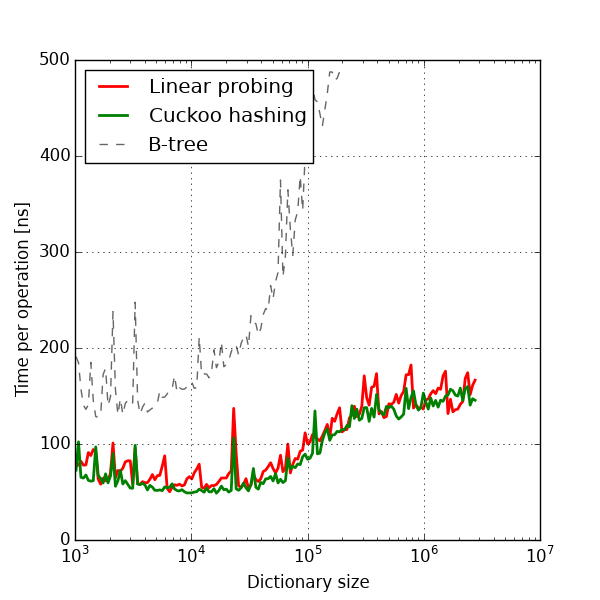
\includegraphics[width=\textwidth]{img/performance/hashing-1}
	\caption{Random \textsc{Find}s}
\end{subfigure}
~
\begin{subfigure}[t]{0.45\textwidth}
	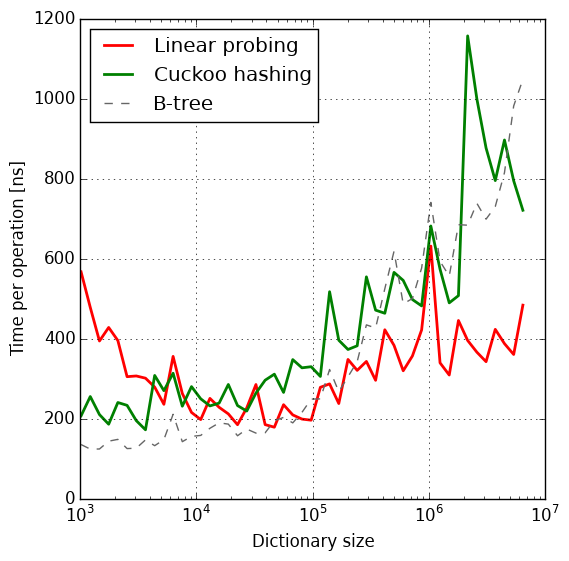
\includegraphics[width=\textwidth]{img/performance/hashing-2}
	\caption{Random \textsc{Insert}s}
\end{subfigure}
\\
\begin{subfigure}[t]{0.45\textwidth}
	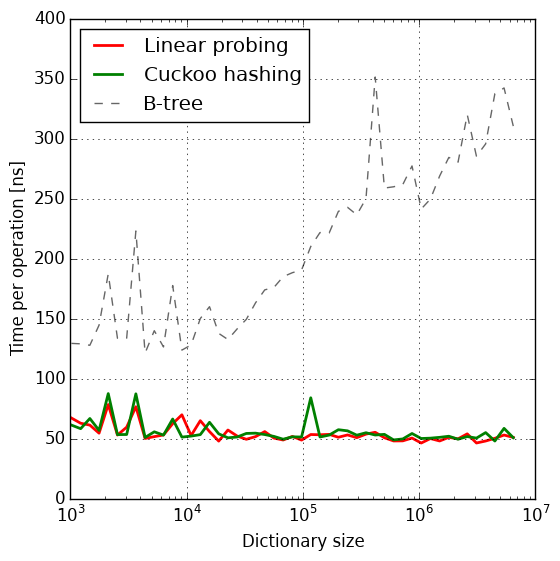
\includegraphics[width=\textwidth]{img/performance/hashing-3}
	\caption{\textsc{Find}s, working set of 1~000 keys}
\end{subfigure}
~
\begin{subfigure}[t]{0.45\textwidth}
	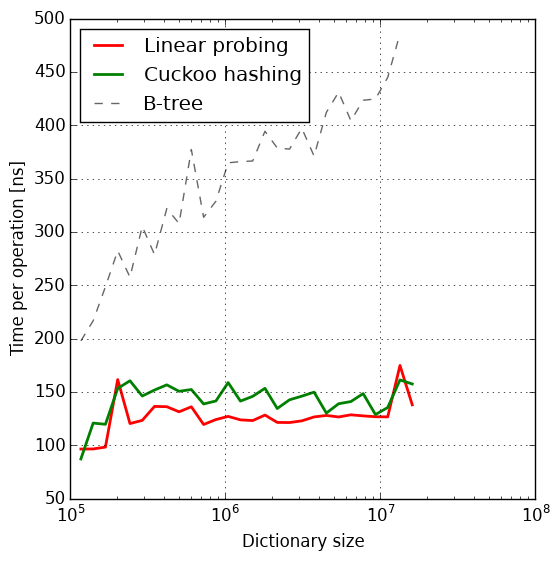
\includegraphics[width=\textwidth]{img/performance/hashing-4}
	\caption{\textsc{Find}s, working set of 100~000 keys}
\end{subfigure}
\caption{Performance of cuckoo hashing and linear probing}
\label{fig:hashing-performance}
\end{figure}

\section{Practical experiments}
\subsection{Mozilla Firefox}
The hash table operations collected from the Firefox session are compressed
in \texttt{data/firefox-htable.tar.gz}. We replayed the operations on all our
dictionary implementations. We normalized the measured times by the maximum
time taken for each recording to allow easier comparison of relative
performance. Our results are presented in Table \ref{tab:firefox-results}.

\begin{table}
\centering
% TODO: Sort!
\begin{tabular}{|c|r|r|r|r|r|r|r|}
	\hline
	Recording &
		B-tree & COBT &
		Splay & $k$-forest & $k$-splay &
		Lin. p. & Cuckoo \\
	\hline
	\texttt{0x7f47930300e0} & 15 & 12 & 14 & 100 & 92 & 6 & \textbf{4} \\
	\hline
	\texttt{0x7fff84eb8f98} & 11 & 14 & 13 & 65 & 100 & 11 & \textbf{6} \\
	\hline
	\texttt{0x7f566e3cb0e0} & 8 & 10 & 10 & 100 & 78 & 9 & \textbf{6} \\
	\hline
	\texttt{0x7fff1d9c7738} & 15 & 15 & 14 & 59 & 100 & 15 & \textbf{6} \\
	\hline
	\texttt{0x7fff84eb9148} & 12 & 14 & 13 & 73 & 100 & 11 & \textbf{7} \\
	\hline
	\texttt{0x7f567b64a830} & 17 & 15 & \textbf{4} & 100 & 70 & 9 & 8 \\
	\hline
	\texttt{0x7f4791631c60} & 12 & 16 & \textbf{9} & 38 & 100 & 17 & 13 \\
	\hline
	\texttt{0x7f47a6e31058} & 11 & 15 & \textbf{9} & 17 & 100 & 23 & 18 \\
	\hline
	\texttt{0x7f5671faab80} & 19 & 28 & \textbf{11} & 19 & 100 & 17 & 22 \\
	\hline
	\texttt{0x7f565ca63148} & \textbf{9} & 12 & 13 & 49 & 100 & 14 & 10 \\
	\hline
	\hline
	Average & 13 & 15 & 11 & 62 & 94 & 13 & 10 \\
	\hline
\end{tabular}
\caption{Results of the Mozilla Firefox experiment. Standardized by maximum
	time (lower is better). Sorted by which implementation is fastest.
	Produced by \texttt{experiments/vcr/make\_table.py}.}
\label{tab:firefox-results}
\end{table}

Overall, the cache-oblivious B-tree (COBT) performed slightly worse than
B-trees in this experiment. We believe this may be explained by the small size
of typical hash tables, which forces frequent costly rebuilds of the packed
memory array.

Most recordings run fastest either on cuckoo hash tables, or on splay trees.
By inspecting the recordings, we found that splay trees are better on recordings
with many updates, while cuckoo tables win when there are much more
\textsc{Find}s. Choosing the wrong structure can reduce the performance,
typically about $2\times$, but, as seen in the case of \texttt{0x7f47930300e0},
the difference can be up to $4\times$.
We believe a data structure that would dynamically switch
its internal representation between cuckoo hashing and splay trees
based on the access pattern may be a good compromise.

Interestingly, linear probing does not behave as well on Firefox recordings
as in synthetic experiments, in which it performed as well as cuckoo hashing
in random \textsc{Find}s and slightly better on \textsc{Insert}s. One possible
reason for this is a higher incidence of failed \textsc{Insert} and
\textsc{Find} operations, which we did not specifically benchmark with
synthetic workloads. While failed \textsc{Find}s on cuckoo hashing take only
2 memory transfers as any other \textsc{Find}, an unsuccessful \textsc{Find}
with linear probing needs to traverse an entire chain.

\subsection{Geospatial database}
The results of the cloud database experiment are outlined in Table
\ref{tab:cloud-results}. Cache-oblivious B-trees slightly outperformed
standard B-trees. Splay trees were surprisingly fast. One factor that might
cause them to perform so well might be that stations usually produce a large
amount of reports over their lifetime, so when we fetch $S$ closest reports
for a point, it is likely that all such reports will be the first $S$ reports
reported by the closest station. Splay trees may thus keep old reports
near the top. In this experiment, we picked $S=1~000$. Also, as can be
seen on Figure \ref{fig:cloud-data}, the distribution of stations on the globe
is very uneven, so stations ``assigned'' to a large area can be kept closer to
the root.

Additionally, we tried two algorithms for sampling query points on the globe.
The first algorithm simply iterated through points on the latitude-longitude
grid with whole number coordinates (i.e.\ -179.0\textdegree W -90.0\textdegree N
through 180.0\textdegree E 90.0\textdegree S).
The second algorithm arbitrarily picked $64~800=180\cdot 360$ random query
points.
The algorithm can be selected by passing different values of the
\texttt{--scatter} flag to \texttt{bin/experiments/cloud}
(\texttt{--scatter=GRID} for grid sampling, or \texttt{--scatter=RANDOM
--samples=64800} for random sampling).

All data structures performed slightly better on the first one, which shows
that more predictable accesses are better for performance. The effect was,
however, comparatively weak on cache-oblivious B-trees.

\begin{table}
\centering
\begin{tabular}{|c|c|c|}
%--close_count=1000
%--scatter=GRID
%--lat_step=100
%--lon_step=100
%--min_year=1997
%--max_year=2005 ===>
%	       dict_cobt:     20 687 539 351 ns
%	      dict_splay:      6 030 131 877 ns
%	     dict_ksplay:     41 687 825 004 ns
%	      dict_btree:     22 677 805 459 ns
%
%--samples=64800 (180*360)
%--scatter=RANDOM ===>
%	       dict_cobt:     20 583 667 067 ns
%	      dict_splay:      6 647 207 153 ns
%	     dict_ksplay:     44 717 377 069 ns
%	      dict_btree:     25 884 347 926 ns
	\hline
	Dictionary & Grid sampling & Random sampling \\
	\hline

	Cache-oblivious B-tree & 20.69 s & 20.58 s \\
	\hline
	Splay tree & 6.03 s & 6.65 s \\
	\hline
	$k$-splay tree & 41.69 s & 44.72 s \\
	\hline
	B-tree & 22.68 s & 25.89 s \\
	\hline
\end{tabular}
\caption{Results of the cloud database experiment, generated
	by \texttt{bin/experiments/cloud --max\_year=2005}.
}
\label{tab:cloud-results}
\end{table}
